
\pdfminorversion=4
\documentclass[xcolor=dvipsnames,fontsize=8pt]{beamer}
\usepackage{tabls}
\usepackage{graphicx}
%\usepackage{animate}
\usepackage{xcolor}

%tikz stuff
\usepackage{tikz}
\usetikzlibrary{shapes.geometric, arrows}
\tikzstyle{startstop} = [rectangle, rounded corners, minimum width=2cm, text
    width=1.8cm, minimum height=1cm,text centered, text=white,draw=black, fill=Gray!140]
\tikzstyle{io} = [trapezium, trapezium left angle=70, trapezium right angle=110,
minimum width=0.5cm, minimum height=1cm, text centered, draw=black,
fill=blue!20!Gray!90!,text=white]
\tikzstyle{process} = [rectangle, minimum width=2cm, minimum height=1cm, text
centered, text width=2cm, draw=black, text=white,fill=Gray!140!blue!70!white]
\tikzstyle{decision} = [diamond, minimum width=3cm, minimum height=1cm, text
centered, draw=black, fill=Gray!,text=white]
\tikzstyle{arrow} = [thick,line width=0.6mm,->,>=stealth]
\tikzstyle{arrow1} = [dashed,->,>=stealth]
\setbeamertemplate{navigation symbols}{}
\setbeamertemplate{footline}[frame number]

%\definecolor{myblue}{rgb}{0.7, 0.7, 60.0}
\definecolor{mylightblue}{rgb}{1,1,1}
\newcommand*{\boxedcolor}{blue}
\newcommand{\bracket}[1]{\left[ #1 \right]}
\newcommand{\bracet}[1]{\left\{ #1 \right\}}
\newcommand{\fn}[1]{\left( #1 \right)}
\newcommand{\ave}[1]{\left\langle #1 \right\rangle}
\newcommand{\norm}[1]{\Arrowvert #1 \Arrowvert}
\newcommand{\abs}[1]{\arrowvert #1 \arrowvert}
\newcommand{\BU}[0]{\ensuremath{\mathbf{U}}}
\newcommand{\BQ}[0]{\ensuremath{\mathbf{Q}}}

\makeatletter
\renewcommand{\boxed}[1]{\textcolor{\boxedcolor}{%
  \fbox{\normalcolor\m@th$\displaystyle#1$}}}
\makeatother
\usepackage{hyperref}

\newcommand{\backupbegin}{
   \newcounter{framenumberappendix}
   \setcounter{framenumberappendix}{\value{framenumber}}
}
\newcommand{\backupend}{
   \addtocounter{framenumberappendix}{-\value{framenumber}}
   \addtocounter{framenumber}{\value{framenumberappendix}} 
}
\renewcommand{\u}[1]{\underline{#1}}

\newcommand{\iso}[2]{${}^{{#2}}${#1} }
\newcommand{\nubar}[0]{$\overline{\nu}$ }
\newcommand{\keff}[0]{\ensuremath{{k}_{\textsf{eff}}} }
\newcommand{\expect}[1]{E[#1] }
\newcommand{\colg}[1]{{\color{ForestGreen} #1}}
\newcommand{\coly}[1]{{\color{yellow} #1}}
\newcommand{\colb}[1]{{\color{blue} #1}}
\newcommand{\colr}[1]{{\color{red} #1}}
\usepackage{amsfonts}
\newlength{\wideitemsep}
\setlength{\wideitemsep}{8pt}
%\addtolength{\wideitemsep}{5pt}
\let\olditem\item
\renewcommand{\item}{\setlength{\itemsep}{\wideitemsep}\olditem}

\newcommand{\N}{\mathbb{N}}
\newcommand{\Z}{\mathbb{Z}}
\newcommand{\deriv}[2]{\frac{\mathrm{d} #1}{\mathrm{d} #2}}
\newcommand{\pderiv}[2]{\frac{\partial #1}{\partial #2}}
\newcommand{\bx}{\mathbf{X}}
\newcommand{\ba}{\mathbf{A}}
\newcommand{\by}{\mathbf{Y}}
\newcommand{\bj}{\mathbf{J}}
\newcommand{\bs}{\mathbf{s}}
\newcommand{\B}[1]{\ensuremath{\mathbf{#1}}}
\newcommand{\Dt}{\Delta t}
\renewcommand{\d}{\mathsf{d}}
\newcommand{\mom}[1]{\langle #1 \rangle}
\newcommand{\xl}{{x_{i-1/2}}}
\newcommand{\xr}{{x_{i+1/2}}}
\newcommand{\il}{{i-1/2}}
\newcommand{\ir}{{i+1/2}}

\AtBeginSection[]
{
    \begin{frame}<beamer>
        \frametitle{Outline}
        \tableofcontents[currentsection]
    \end{frame}
}

\setbeamerfont{frametitle}{size=\Large}
\setbeamerfont{normal font}{size=\tiny}

\graphicspath{{figures/}}

\usepackage{verbatim}
\usepackage{comment}
\usepackage[]{datetime}
\usepackage{multirow}

\newcommand{\thedate}{\today}


\setlength{\tabcolsep}{1.05cm}
\geometry{paperwidth=140mm,paperheight=105mm}

%Aggie-themed
\pgfdeclareimage[height=0.1in]{TAMUlogo}{tamu_engineering.png}
\logo{\raisebox{-8pt}{\pgfuseimage{TAMUlogo}}}
\titlegraphic{\centering\begin{tabular}{c}

\includegraphics[height=0.18\textheight]{tamu_seal.png}\end{tabular}}
%Michigan-themed
%\pgfdeclareimage[height=0.1in]{UMlogo}{michigan_engineering.png}
%\logo{\raisebox{-8pt}{\pgfuseimage{UMlogo}}}
%\titlegraphic{
\includegraphics[height=0.2\textheight]{michigan_block_m.png}}


%%%%%%%%%%%%%%%%%%%%%%%%%%%%%%%%%%%%%%%%%%%%%%%%%%%%%%%%%%%%%%%
% Optional packages, used to show off certain tricks

\newlength \figwidth
\setlength \figwidth {0.5\textwidth}

\setlength{\leftmargin}{-2cm}
\setlength{\rightmargin}{-2cm}

%%%%%%%%%%%%%%%%%%%%%%%%%%%%%%%%%%%%%%%%%%%%%%%%%%%%%%%%%%%%%%%

\usepackage[english]{babel}
\usetheme{Frankfurt}

%Make it Aggie Maroon
\usecolortheme[RGB={80,0,0}]{structure}  
%Or Michigan Blue
%\usecolortheme[RGB={0,0,153}]{structure}  
%Or Michigan Maize
%\usecolortheme[RGB={255,204,0}]{structure}  

  % This will typeset only the frames (or slides) that have the given label ("current" in this case).

\title{Second-Order Discretization in Space and Time for Grey S$_2$-Radiation Hydrodynamics}
    \author{{\large Simon R. Bolding, Joshua E. Hansel, \& Jim E. Morel}}
\date{16 October 2015 \\ \vspace{0.05in} {CLASS seminar}}
\subject{}
%\institute{Los Alamos National Laboratory}

% \classificationlevel{SECRET/RD}
% \transmissible{}

%\reportnum{\textcolor{blue}{SAMPLE TEMPLATE ONLY \\ Contains NO Classified
%Information}}

%\dissableframenumber
\begin{document}

\begin{frame}
    \titlepage \vspace{-0.213in}
    \begin{center}
    \end{center}    
\end{frame}

\setlength{\tabcolsep}{6pt}

\begin{frame}
\frametitle{Outline}
\begin{minipage}{0.061\linewidth}
\hfill                      
\end{minipage}
\begin{minipage}{0.8\linewidth}
\tableofcontents[
hideothersubsections,
sectionstyle=show,
subsectionstyle=hide
]
\end{minipage}

\end{frame}


\section{Overview}
\subsection{}

\begin{frame}
    \frametitle{What is radiation hydrodynamics?}
    \begin{itemize}
        \item Thermal radiative transfer coupled to material motion
            \begin{itemize}
                \item Inertial confinement fusion (NIF) and astrophysics calculations
            \end{itemize}
    \end{itemize}
    \begin{figure}
    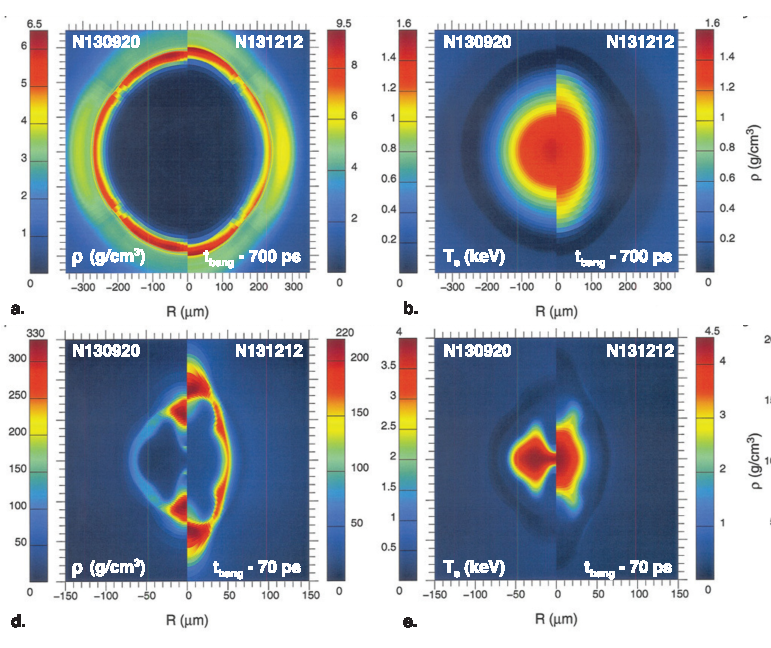
\includegraphics[width=0.8\textwidth,trim=0.1in 0.1in 0.0in 0.1in,clip]{nif.pdf}
    \caption{Comparison of HYDRA simulations for collapses of 2 NIF hohlraum designs, from Meezan et.
    al., 2015}
    \end{figure}
\end{frame}

\begin{frame}
    \frametitle{Example of a 1D Radiative Shock Solution}
    \begin{block}{Goal of this project}
        \begin{itemize}
            \item
     Extended work by Edwards and Morel for a method that is second-order in
     \colb{space} and \colb{time}
 \item We extended the method to S$_2$ equations which allows for conservation of momentum 
     \begin{itemize}
        \item Can be generalized to S$_n$ equations, but would require some form of
            acceleration
     \end{itemize}
     \end{itemize}
 \end{block}
\end{frame}

\begin{frame}
    \frametitle{The hydrodynamics equations}
    \begin{itemize}
        \item The 1D Euler Equations
            \begin{equation}a
                \pderiv{ }{t}\BU + \pderiv{ }{x}f(U) = \mathbf{Q}
            \end{equation}

    \end{itemize}

\end{frame}

\begin{frame}
    \frametitle{The hydrodynamics equation governing equations continued}
    \begin{itemize}
    \item Radiation transport equation, collocated to $\mu=\pm\frac{1}{\sqrt{3}}$
        \begin{equation*}
\frac{1}{c}\pderiv{\psi^\pm}{t} \pm \frac{1}{\sqrt{3}}\pderiv{\psi^\pm}{x} + \sigma_t
\psi^\pm = 
\frac{\sigma_s}{4\pi} cE_r + \frac{\sigma_a}{4\pi} acT^4  - \frac{\sigma_t u}{4\pi c}
F_{r,0} \pm  
\frac{\sigma_t}{\sqrt{3}\pi}E_r u 
\end{equation*} 
    \item
\end{itemize}
\end{frame}


\begin{frame}
    \frametitle{The MUSCL Hancock method}
    \begin{itemize}
    \item The MUSCL Hancock method is a finite volume method that utitlized
        slope-reconstruction in space

        PICTURE OF SLOPE RECONSTRUCTION

    \item A predictor corrector in time is used for second order accuracy
    \item For example, from $t_n$ to $t_{n+1/2}$
        \begin{itemize} 
            \item Step 1
        \begin{equation*}
            U^* = U^n + \frac{\Dt}{4}(F(U^n))
        \end{equation*}
            \item Step 2
        \begin{equation*}
            U^{N+1} = U^n + \frac{\Dt}{2}(F(U^*))
        \end{equation*}
        \end{itemize}
    \end{itemize}
\end{frame}

\begin{frame}
    \frametitle{Linear Discontinuous Galerkin Spatial Discreziation for TRT}
    \begin{itemize}
    \item We use a lumped linear discontinous trial space representation, with upwinding.
\item There is no slope reconstruction
\item Preserves the equilibrium diffusion limit


\end{itemize}


\end{frame}

\begin{frame}
    \frametitle{Operator splitting and general approach}
\end{frame}

\begin{frame}
    \frametitle{Development of Algorithm}


\end{frame}


\begin{frame}
    \frametitle{Non-linear iteration scheme for implicit solve} 


\end{frame}

\begin{frame}
    \frametitle{Extra stuff}
    Code implemented in python

    Energy slope stuff

    Other things


\end{frame}

\begin{frame}
    \frametitle{Future Work}

    Coupling to a high-order system using hybrid-``S$_2$-like'' equations.
\end{frame}



\section{High-Order Solver}
\subsection{}


\begin{frame}
    \frametitle{Space-Angle LDFE Mesh}
    \noindent
    \fontsize{9.89}{5.0}\selectfont
    \begin{minipage}[t]{0.36\linewidth}
        \centering
        \scalebox{0.8}{
        \begin{tikzpicture}
            \draw (1,1) rectangle (4,4);
            \node[draw,circle,inner sep=1.2 pt,fill] at (2.5,2.5) {};
            \node[above] at (2.5,2.5) {$(x_i,\mu_j)$};
            \draw (1.0,0.4) -- (1.0,0.6) node[below, pos=0.4] {$x_{i-1/2}$};
            \draw (4.0,0.4) -- (4.0,0.6) node[below, pos=0.4] {$x_{i+1/2}$};
            \draw (0.4,1.0) -- (0.6,1.0) node[left, pos=0.4] {$\mu_{j-1/2}$};
            \draw (0.4,4.0) -- (0.6,4.0) node[left, pos=0.4] {$\mu_{j+1/2}$};
            \draw [thick,->] (0.5,0.5) -- (5,0.5) node[anchor=north west] {$x$};
            \draw [thick,->] (0.5,0.5) -- (0.5,5) node[anchor=east] {$\mu$};
        \end{tikzpicture}
    }
    \end{minipage}%
    \begin{minipage}[t]{0.70\linewidth}
        \vspace{-1.6in}
        \hspace{0.5in}
        \begin{itemize}
            \item {\small $\displaystyle \tilde \psi(x,\mu)$} is linear over each
                cell, \colb{preserving} $0^{\text{th}}$ and $1^{\text{st}}$ moment in $x$
                and $\mu$
            \item Use path-length estimators of flux to approximate moments e.g.
            {\small
            \begin{align*}
                \mom{\psi}_{\mu,ij} &= \frac{6}{h_{\mu}^2h_x}
             \iint\limits_\mathcal{D} (\mu-\mu_i) \psi(x,\mu) \d x \d \mu 
        \end{align*}}    
        \end{itemize}
    \end{minipage}
    \pause
    \begin{itemize}
       \item Use standard LD and upwinding to get face terms
    \end{itemize}
\end{frame}



\date{16 October 2015}

\begin{frame}
    \frametitle{{\LARGE\coly{Questions?}}}
    \titlepage \vspace{-0.113in}
\end{frame}

\backupbegin
\appendix

\title{Backup Slides}
\author{}
\date{}

\begin{frame}
    \frametitle{The full equations}
    \begin{itemize}
        \item Material balance equations
\begin{align*}
\pderiv{\rho}{t}+\pderiv{}{x}\fn{\rho u} &= 0 \\
\pderiv{}{t}\fn{\rho u} + \pderiv{}{x}\fn{\rho u^2 + p} &=
\frac{\sigma_t}{c} F_{r,0} \\
\pderiv{E}{t} + \pderiv{}{x}\bracket{\fn{E+p}u} &= -\sigma_a c \fn{aT^4 -
E_r}+\frac{\sigma_t u}{c} F_{r,0} 
\end{align*}
    \item Radiation transport equation, collocated to $\mu=\pm\frac{1}{\sqrt{3}}$
        \begin{equation*}
\frac{1}{c}\pderiv{\psi^\pm}{t} \pm \frac{1}{\sqrt{3}}\pderiv{\psi^\pm}{x} + \sigma_t
\psi^\pm = 
\frac{\sigma_s}{4\pi} cE_r + \frac{\sigma_a}{4\pi} acT^4  - \frac{\sigma_t u}{4\pi c}
F_{r,0} \pm  
\frac{\sigma_t}{\sqrt{3}\pi}E_r u 
\end{equation*}
\end{itemize}
\end{frame}




\backupend
\end{document}

